\section{Технический проект}
\subsection{Общая характеристика организации решения задачи}

Необходимо спроектировать и разработать сайт-форум для обсуждения на нём различных тем.


Веб-сайт — это комплекс взаимосвязанных электронных страниц, сгруппированных в разделы и доступных через уникальный интернет-адрес в форме www.имя\_сайта.ru. Каждая страница веб-сайта представляет собой текстовый документ, созданный с применением различных языков программирования, таких как HTML, CSS, JavaScript и другие.

\subsection{Обоснование выбора технологии проектирования}

На сегодняшний день информационный рынок, поставляющий программные решения в выбранной сфере, предлагает множество продуктов, позволяющих достигнуть поставленной цели – разработки web-сайта.

\subsubsection{Описание используемых технологий и языков программирования}

В процессе разработки web-сайта используются программные средства и языки программирования. Каждое программное средство и каждый язык программирования применяется для круга задач, при решении которых они необходимы.

\subsubsection{Язык программирования Python}

Python – это интерпретируемый, высокоуровневый язык программирования с динамической типизацией, который обеспечивает простоту в использовании, читаемость кода и эффективное взаимодействие с другими языками и системами. Основное предназначение данного языка – это создание серверной части веб-приложения, обеспечивая взаимодействие с веб-сервером. Это позволяет обрабатывать HTTP-запросы, управлять сессиями и осуществлять обработку данных от клиентов, а также взаимодействовать с базой данных.

\subsubsection{Язык программирования JavaScript}

\paragraph{Достоинства языка JavaScript}

JavaScript – это высокоуровневый, интерпретируемый язык программирования, который широко используется для создания интерактивных и динамичных веб-сайтов. Разработанный Netscape, JavaScript стал ключевым компонентом веб-технологий, позволяя веб-страницам взаимодействовать с пользователем, изменять содержимое и обеспечивать богатый пользовательский опыт. JavaScript используется для создания интерактивных элементов пользовательского интерфейса на веб-сайтах форумов. Это включает в себя динамическую подгрузку данных, анимации, обработку событий и обновление содержимого страницы без ее перезагрузки. JavaScript может обеспечивать валидацию данных, введенных пользователями в формах, перед отправкой на сервер. Также он применяется для асинхронного взаимодействия с сервером, например, для отправки комментариев, без необходимости перезагрузки всей страницы. JavaScript позволяет динамически обновлять содержимое форума в реальном времени. Это может включать в себя добавление новых тем, обновление сообщений, и другие изменения, которые пользователь может видеть без необходимости обновления всей страницы. JavaScript используется для взаимодействия с серверной частью, осуществляя запросы к API форума на Python. Это включает передачу данных между клиентом и сервером, а также обновление интерфейса в соответствии с полученными данными.

\paragraph{Недостатки языка Javascript}

JavaScript может вести себя по-разному в различных браузерах, что создает проблемы с кросс-браузерной совместимостью. Некоторые функции могут работать по-разному или вовсе отсутствовать в различных браузерах, что требует дополнительного тестирования и учета особенностей при разработке. JavaScript выполняется на стороне клиента, и поэтому пользователи могут иметь доступ к исходному коду и внести изменения. Это может создавать уязвимости безопасности, такие как внедрение вредоносного кода или модификация данных на стороне клиента. По соображениям безопасности JavaScript имеет ограниченный доступ к файловой системе клиентского устройства. Это может затруднить реализацию некоторых функций, таких как загрузка и сохранение файлов на стороне клиента. Средства отладки JavaScript в браузере могут быть менее мощными и удобными, чем средства отладки на сервере. Это может затруднить выявление и устранение ошибок в коде JavaScript. Обработка ошибок в JavaScript иногда может быть неочевидной из-за асинхронной природы языка. Это может затруднить выявление и отладку ошибок, особенно в сложных веб-приложениях.

\subsection{Диаграмма компонентов и схема обмена данными между файлами компонента}

Диаграмма компонентов описывает особенности физического представления разрабатываемой системы. Она позволяет определить архитектуру системы, установив зависимости между программными компонентами, в роли которых может выступать как исходный, так и исполняемый код. Основными графическими элементами диаграммы компонентов являются компоненты, интерфейсы, а также зависимости между ними. На рисунке \ref{comp:image} изображена диаграмма компонентов для проектируемой системы. Она включает в себя сервер с операционной системой, на которой установлена система управления содержимым, включающая в себя базу данных и интерфейс. Помимо этого на диаграмме изображен клиентский компьютер с операционной системой, на которой установлен браузер.

\begin{figure}[ht]
\center{\includegraphics[width=1\linewidth]{comp}}
\caption{Диаграмма компонентов}
\label{comp:image}
\end{figure}

Любой компонент должен быть вызван в сценарии страницы web-сайта. Web-страница передает данные компоненту в момент вызова последнего.

На рисунке \ref{data:image} представлена схема обмена данными между сценариями компонента при вызове компонента на странице сайта.

\begin{figure}[ht]
\center{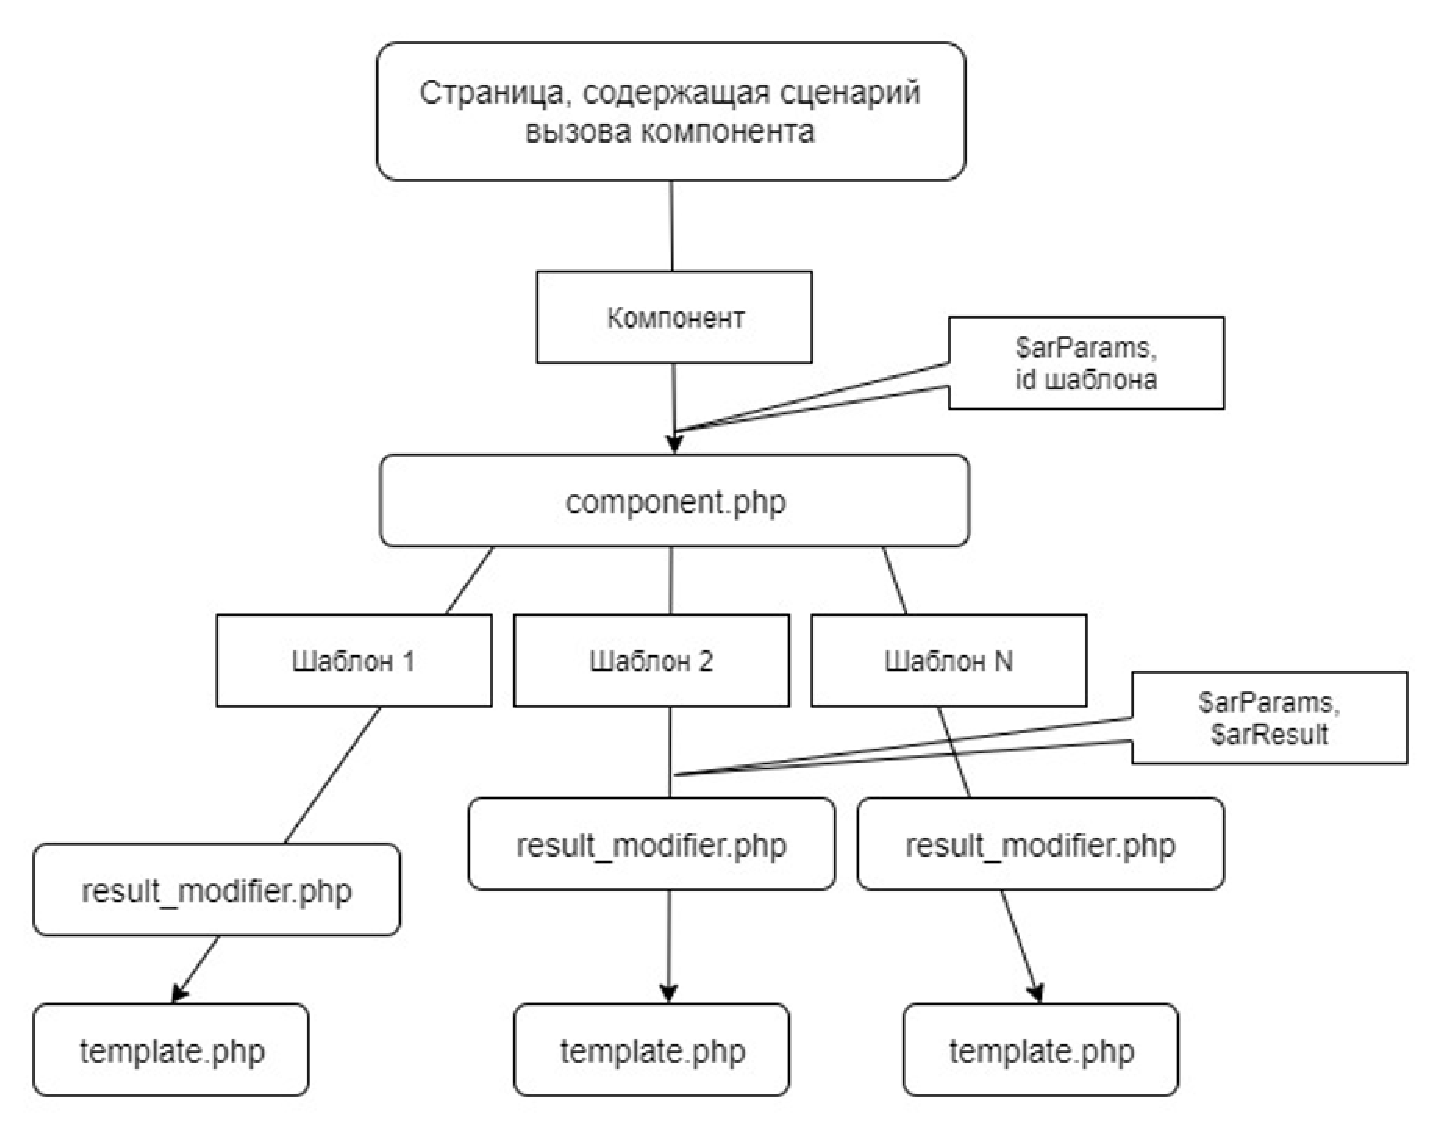
\includegraphics[width=1\linewidth]{data}}
\caption{Диаграмма компонентов}
\label{data:image}
\end{figure}

При вызове компонента в сценарии web-страницы указываются значения параметров компонента, которые далее посредством массива \$arParams передаются в сценарий файла component.php.

В сценарии файла component.php посредством метода \linebreak IncludeComponentTemplate класса CBitrixComponent происходит вызов одного из шаблонов компонента. Id шаблона также определяется в сценарии страницы web-приложения и неявно для разработчика передается указанный выше метод. Подключается сценарий файла template.php одного из шаблонов, в который передается, возможно, измененный в сценарии component.php массив \$arParams и, также, сформированный в сценарии component.php массив \$arResult. Оба этих массива доступны также и в файле result\_modifier.php, который подключается перед подключением файла template.php. 

Работа компонента заканчивается в момент завершения работы сценария файла component.php, т.е. возможно выполнить действия уже после подключения шаблона. Однако, если массив \$arResult будет изменен в сценарии шаблона, в сценарий файла компонента component.php измененные данные переданы не будут.

\subsection{Диаграмма размещения}

Диаграмма размещения (рис.~\ref{place:image}) отражает физические взаимосвязи между программными и аппаратными компонентами системы.

\vspace{-8mm} % чтобы убрать пустую строку, которая осталась после переноса рисунка на следующую страницу
\begin{figure}[ht]
\center{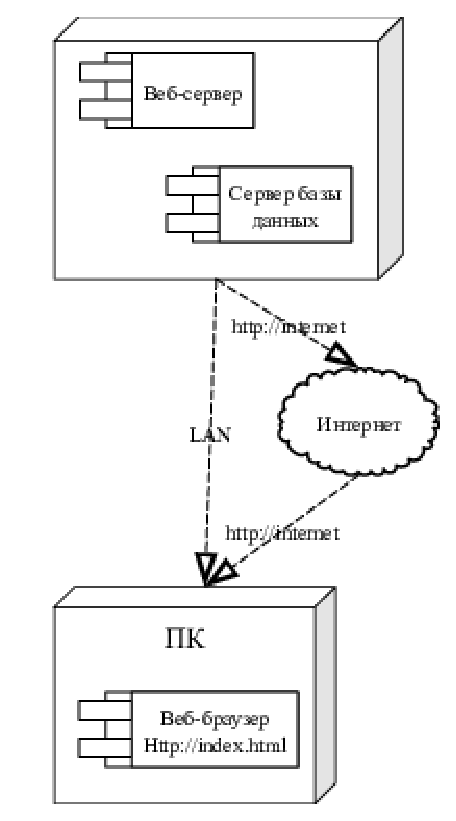
\includegraphics[width=0.57\linewidth]{place}}
\caption{Диаграмма размещения. Не помещается на страницу. Очень длинный заголовок}
\label{place:image}
\end{figure}

Она является хорошим средством для показа маршрутов перемещения объектов и компонентов в распределенной системе.

В таблице \ref{ssevsws:table} приведен пример использования пакета xltabular с автоматическим расчетом ширины столбца.

\begin{xltabular}{\textwidth}{|c|X|X|}
	\caption{Сравнение протоколов SSE и WebSocket\label{ssevsws:table}}\\ \hline
	~  & \centrow  SSE & \centrow WebSocket \\ \hline
	\endfirsthead
	\continuecaption{Продолжение таблицы \ref{ssevsws:table}}
	~ & \centrow SSE & \centrow WebSocket \\ \hline 
	\finishhead
	Направленность & 
	Однонаправленный, полудуплексный: данные посылает только сервер & 
	Двунаправленный, полнодуплексный: и сервер, и клиент могут обмениваться сообщениями \\ \hline 
	Соединение  & HTTP & WS \\ \hline 
	Тип данных & Только текст & Бинарные и текстовые данные \\ \hline 
	Доп. возможности & Встроенный механизм идентификаторов событий и переподключения & Переподключение и идентификация события реализуются на стороне приложения
\end{xltabular}

\subsection{Содержание информационных блоков. Основные сущности}

Проанализировав требования, можно выделить шесть основных сущностей:
\begin{itemize}
\item "<Новости">;
\item "<Продукция">;
\item "<Услуги">.
\end{itemize}

В состав сущности "<Новости"> можно включить атрибуты, представленные в таблице \ref{news:table}.

\begin{xltabular}{\textwidth}{|l|l|p{1.7cm}|X|}
	\caption{Атрибуты сущности "<Новости">\label{news:table}}\\ \hline
	\centrow Поле & \centrow Тип & \centrow Обяза\-тельное & \centrow Описание \\ \hline
	\thead{1} & \thead{2} & \centrow 3 & \centrow 4 \\ \hline
	\endfirsthead
	\continuecaption{Продолжение таблицы \ref{news:table}}
	\thead{1} & \thead{2} & \centrow 3 & \centrow 4 \\ \hline
	\finishhead
	\_id & ObjectId & true & Уникальный идентификатор \\ \hline 
	head & String & true & Заголовок новости \\ \hline 
	short & String & false & Аннотация к новости \\ \hline 
	createdAt & Date & true & Время создания новости \\ \hline 
	author & String & false & Автор новости \\ \hline 
	content & String & true & Текст новости \\ \hline 
	views & Integer & true & Количество просмотров новости зарегистрированными пользователями
\end{xltabular}

Пример использования различных типов столбцов представлен в таблице \ref{prod:table}. Рекомендуется использовать пакет xltabular для создания таблиц.

\begin{xltabular}{\textwidth}{|R|C{2.5cm}|l|T|}
	\caption{Атрибуты  сущности "<Новости разметки в LaTeX"> с использованием различных типов столбцов и многострочным заголовком\label{prod:table}}\\ \hline
	\centrow Поле & \centrow Тип & \centrow Обязательное & \centrow Описание \\ \hline
	\centrow 1 & \centrow 2 & \thead{3} & \centrow 4 \\ \hline
	\endfirsthead
	\continuecaption{Продолжение таблицы \ref{prod:table}}
	\centrow 1 & \centrow 2 & \thead{3} & \centrow 4 \\ \hline
	\finishhead
	\_id & ObjectId & true & Уникальный идентификатор \\ \hline 
	head & String & true & Заголовок новости \\ \hline 
	short & String & false & Аннотация к новости \\ \hline 
	createdAt & Date & true & Время создания новости \\ \hline 
	author & String & false & Автор новости \\ \hline 
	content & String & true & Текст новости \\ \hline 
	views & Integer & true & Количество просмотров новости зарегистрированными пользователями
\end{xltabular}

В системе предусмотрен внутренний механизм связи между разделами и элементами информационных блоков, поэтому введения дополнительных идентификаторов при реализации связей между сущностями не предполагается.

Экземпляры сущностей реализуются в информационных блоках посредством элементов, атрибуты сущности – посредством полей и свойств элемента. 
